% Created 2025-02-25 ter 09:15
% Intended LaTeX compiler: lualatex
\documentclass[presentation,professionalfonts,aspectratio=169]{beamer}
                

% 
\makeatletter
 \@ifclassloaded{beamer}{%
  %%% save beamer's `solution' environment as `beamersolution':
  \let\beamersolution\solution
  \let\endbeamersolution\endsolution
  %%% "delete" the `solution' environment:
  \let\solution\relax
  \let\endsolution\relax
}{%
}%
\makeatother
\usepackage[utf8]{inputenc}
\usepackage[T1]{fontenc}
%\usepackage[french]{babel}
\usepackage[portuguese]{babel}

%%%% FONTS




\usepackage{xsim}
\usepackage[most]{tcolorbox}
\usepackage{amssymb}
\usepackage{fontawesome}
\newcounter{paragraph}



\DeclareExerciseEnvironmentTemplate{custom}{%
  \begin{tcolorbox}[boxrule = 0pt]
  \tcbox[on line,colback=teal,colframe=teal,coltext=white,size=small]{%
    \faBook\sffamily\bfseries\
    \XSIMmixedcase{\GetExerciseName}
    \GetExerciseProperty{counter}%
  }\quad
}{\end{tcolorbox}}


\DeclareExerciseEnvironmentTemplate{custom2}{%
  \begin{tcolorbox}[boxrule = 0pt]
  \tcbox[on line,colback=violet,colframe=violet,coltext=white,size=small]{%
    \faToggleOn\sffamily\bfseries\
    \XSIMmixedcase{\GetExerciseName}
    \GetExerciseProperty{counter}%
  }\quad
}{\end{tcolorbox}}




\DeclareExerciseType{test}{
	exercise-env = question ,
	solution-env = answer ,
	exercise-template = custom ,
	solution-template = custom2 ,
	exercise-name	= Exemplo. ,
	exercises-name = Exemplo ,
	solution-name = Solução ,
	solutions-name = Sol. ,
	exercise-heading = \textbf ,
	solution-heading = \textbf
}


\xsimsetup{
  exercise/within = section,
  exercise/the-counter =  \arabic{exercise}, 
%%solution-name = solution,  % used with headings=true
solution/print=false,
%print-collection/print=both,
}





\usepackage{colortbl}
\usepackage[tikz]{bclogo}
\usetikzlibrary{fit,patterns,shadows.blur,shapes,mindmap}
\usetikzlibrary{arrows,calc,arrows.meta,decorations.markings,shapes.symbols}
\usetikzlibrary{decorations.pathreplacing, decorations.pathmorphing,calc,arrows,positioning}
\usepackage{tikzpeople}
\usepackage{qrcode,hyperref}
\usepackage{upgreek}
%\usepackage[version=4]{mhchem}
\usepackage{tabularray}


\NewTblrTheme{fancy}{
\SetTblrStyle{caption-tag}{font=\bfseries}
\SetTblrInner[tblr,longtblr]{rowsep=2.5pt}
\DefTblrTemplate{firsthead, middlehead,lasthead}{default}{} % <---
\DefTblrTemplate{contfoot-text}{normal}{\scriptsize\textit{Continued on the next page}}
\SetTblrTemplate{contfoot-text}{normal}
}






\usepackage{chemfig,chemmacros,elements,chemformula}
\chemsetup{modules={all}}
\chemsetup[redox]{pos=top,roman=false}
\chemsetup[redox]{pos=top}
\chemsetup{redox/sep=.5em}
\chemsetup[redox]{explicit-sign=true}
\NewChemPhase\lqdd{\(\ell\)}
\NewChemPhase\gr{grafite}
\NewChemPhase\reac{reação}
\NewChemState\Enthalpy{symbol=H,superscript=,unit=\kilo\joule}%
\usepackage{siunitx}
\setchemfig{fixed length=false, atom sep=2.5em, arrow offset=6pt, scheme debug=false}%,angle increment=30}
\renewcommand*\printatom[1]{\ensuremath{\mathsf{#1}}} % This line changes the font of the atoms to sans serif
%%%% QRCODE
\usepackage{pdfpages}
\usepackage{mol2chemfig}
\usepackage{subfig,caption}
\usepackage{wrapfig}
\usepackage{enumitem}
\setitemize{label=\usebeamerfont*{itemize item}%
\usebeamercolor[fg]{itemize item}
\usebeamertemplate {itemize item}}
\usepackage{array} % ajust colunm table
\usepackage{cancel}
\usepackage[controls]{animate}
\renewcommand{\CancelColor}{\color{red}}

%%%%%%%%%%%%%%%%%%% CONFIG TCOLORBOX 

\newtcolorbox{mybox}[2][]{boxsep=0.5em,left=0.5em,
colback=blue!5!white, colframe=blue!75!black,
fonttitle=\bfseries\sffamily,
colbacktitle=blue!85!red!60,enhanced,
attach boxed title to top left={yshift=-3mm,xshift=5mm},
title=#2,#1}

\newtcolorbox{myrule}[2][]{boxsep=0.5em,left=0.5em,
colback=green!5!white, colframe=blue!75!black,
fonttitle=\bfseries\sffamily,
colbacktitle=blue!85!red!60,enhanced,
attach boxed title to top left={yshift=-3mm,xshift=5mm},
title=#2,#1}


\newtcolorbox{myex}[2][]{boxsep=0.5em,left=0.5em,
  colback=yellow!5!white, colframe=blue!75!black, 
  fonttitle=\bfseries\sffamily,
  colbacktitle=blue!85!red!60,enhanced,
  attach boxed title to top left={yshift=-3mm,xshift=5mm},
  title=#2,#1}


 \definecolor{col1}{HTML}{FF7878}
 \definecolor{col2}{HTML}{51B5F8}
 \definecolor{col3}{HTML}{68E1AA}
 \definecolor{col4}{HTML}{B869EA}
 \definecolor{col5}{HTML}{FF5500}
 \definecolor{col6}{HTML}{FFF8E7}
 \definecolor{col7}{HTML}{FF9966}
 \definecolor{col8}{HTML}{9400D3}



\definesubmol\nobond{-[,0.2,,,draw=none]\scriptstyle\color{blue}}
\newcommand{\re}{\hspace{-1cm}}
\newcommand{\af}{\hspace{2cm}}

%%%% Config X sim for BEAMER
\usepackage{ragged2e}
\justifying
\makeatletter
\@ifclassloaded{beamer}{%
%%% save beamer's `solution' environment as `beamersolution':
\let\beamersolution\solution
\let\endbeamersolution\endsolution
%%% "delete" the `solution' environment:
\let\solution\relax
\let\endsolution\relax
}{%
}%
\makeatother
\usepackage[utf8]{inputenc}
\usepackage[T1]{fontenc}
%\usepackage[portuguese, ]{babel}
%\usepackage[br]{pgf-PeriodicTable}
%%%% FONTS
%%% XSIM CONFIG BEAMER
\usepackage{xsim}
\usepackage{amsmath}
\usepackage[most]{tcolorbox}
\usepackage{amssymb}
\usepackage{fontawesome}
\usepackage{tasks}
\newcounter{paragraph}
%\usepackage[dvipsnames,svgnames]{xcolor}
\usepackage[dvipsnames]{xcolor}
%\usepackage{annotate-equations}
%%% BOX EXERCISE BEAMER
\DeclareExerciseEnvironmentTemplate{custom}{%
\begin{tcolorbox}[boxrule = 0pt]
\tcbox[on line,colback=teal,colframe=teal,coltext=white,size=small]{%
\faBook\sffamily\bfseries\
\XSIMmixedcase{\GetExerciseName}
\GetExerciseProperty{counter}%
}\quad
}{\end{tcolorbox}}
%% == CUSTOM BOX BEAMER
\DeclareExerciseEnvironmentTemplate{custom2}{%
\begin{tcolorbox}[boxrule = 0pt]
\tcbox[on line,colback=violet,colframe=violet,coltext=white,size=small]{%
\faToggleOn\sffamily\bfseries\
\XSIMmixedcase{\GetExerciseName}
\GetExerciseProperty{counter}%
}\quad
}{\end{tcolorbox}}
\DeclareExerciseType{test}{
exercise-env = question ,
solution-env = answer ,
exercise-template = custom ,
solution-template = custom2 ,
exercise-name = Exemplo ,
exercises-name = Exemplo ,
solution-name = Solução ,
solutions-name = Sol. ,
exercise-heading = \textbf ,
solution-heading = \textbf
}
\xsimsetup{
exercise/within = section,
exercise/the-counter =  \arabic{exercise},
%%solution-name = solution,  % used with headings=true
solution/print=true,
print-collection/print=both,
}
\NewTasksEnvironment[label = (\emph{\alph*}),
label-width = 12pt]{choice}[\choice]
\usepackage{empheq} %%% Brackers
\usepackage{colortbl}
\usepackage[tikz]{bclogo}
\usetikzlibrary{calc,fadings,shadings}
\usetikzlibrary{fit,patterns,shadows.blur,shapes,mindmap}
\usetikzlibrary{arrows,snakes,shapes,arrows.meta,decorations.markings,shapes.symbols}
\usetikzlibrary{backgrounds,shapes.geometric}
\usetikzlibrary{decorations.pathreplacing, decorations.pathmorphing,arrows,positioning}
\usepackage{tikzpeople}
\usepackage{qrcode,hyperref}
\usepackage{upgreek}
%\usepackage[version=4]{mhchem}
\usepackage{tabularray}
%%% PACKAGE PLOT GRAPH
\usepackage{pgfplots}
\pgfplotsset{width=10cm,compat=1.9}
%%% CUSTOM TABLE
\NewTblrTheme{fancy}{
\SetTblrStyle{caption-tag}{font=\bfseries,red2}
\SetTblrInner[tblr,longtblr]{rowsep=2.5pt}
\DefTblrTemplate{firsthead, middlehead,lasthead}{default}{} % <---
\DefTblrTemplate{contfoot-text}{normal}{\scriptsize\textit{Continua ...}}
\SetTblrTemplate{contfoot-text}{normal}
}
%% ==== CHEMMACROS E CHEMFIG CONFIG
\usepackage{chemfig,chemmacros,elements,chemformula}
\chemsetup{modules={all}}
\chemsetup[redox]{pos=top,roman=false}
\chemsetup[redox]{pos=top}
\chemsetup{redox/sep=.5em}
\chemsetup[redox]{explicit-sign=true} %%% reaction redox
%% == CUSTOM PHASES IN CHEMMACROS
\NewChemPhase\lqdd{\(\ell\)}
\NewChemPhase\gr{grafite}
\NewChemPhase\reac{reação}
\NewChemState\Enthalpy{symbol=H,superscript=,unit=\kilo\joule\per\mole}%
\NewChemState\Entalpia{symbol=H,superscript=,unit=\kilo\cal\per\mole}%
\usepackage{siunitx}
\setchemfig{fixed length=false, atom sep=2.5em, arrow offset=6pt, scheme debug=false}
%% == NUMEROS PARA FORMULES
\renewcommand*\printatom[1]{\ensuremath{\mathsf{#1}}} % This line changes the font of the atoms to sans serif
%%% INCLUDE PAGES PDFs
\usepackage{pdfpages}
\usepackage{mol2chemfig}
\usepackage{xymtexpdf}
%\changeunitlength{0.08pt}
%%\wedgehasheddash
\usepackage{subfig,caption}
\usepackage{wrapfig}
\usepackage{enumitem}
\setitemize{label=\usebeamerfont*{itemize item}%
\usebeamercolor[fg]{itemize item}
\usebeamertemplate {itemize item}}
\usepackage{array} % ajust colunm table
\usepackage{cancel}
%%%% ---------- FILMES AND ANIMATIONS
\usepackage[controls]{animate}
%\usepackage{movie15}
\usepackage{media9}
\renewcommand{\CancelColor}{\color{red}}
%%%%%%%%%%%%%%%%%%% CONFIG TCOLORBOX
\newtcolorbox{mybox}[2][]{boxsep=0.5em,left=0.5em,
colback=blue!5!white, colframe=blue!75!black,
fonttitle=\bfseries\sffamily,
colbacktitle=blue!85!red!60,enhanced,
attach boxed title to top left={yshift=-3mm,xshift=5mm},
title=#2,#1}
\newtcolorbox{myrule}[2][]{boxsep=0.5em,left=0.5em,
colback=green!5!white, colframe=blue!75!black,
fonttitle=\bfseries\sffamily,
colbacktitle=blue!85!red!60,enhanced,
attach boxed title to top left={yshift=-3mm,xshift=5mm},
title=#2,#1}
\newtcolorbox{myex}[2][]{boxsep=0.5em,left=0.5em,
colback=yellow!5!white, colframe=blue!75!black,
fonttitle=\bfseries\sffamily,
colbacktitle=blue!85!red!60,enhanced,
attach boxed title to top left={yshift=-3mm,xshift=5mm},
title=#2,#1}
\tcbset{colback=yellow!10!white, colframe=red!50!black, highlight math style= {enhanced, %<-- needed for the ’remember’ options
colframe=red,colback=red!10!white,boxsep=0pt}}
\definecolor{col1}{HTML}{FF7878}
\definecolor{col2}{HTML}{51B5F8}
\definecolor{col3}{HTML}{68E1AA}
\definecolor{col4}{HTML}{B869EA}
\definecolor{col5}{HTML}{FF5500}
\definecolor{col6}{HTML}{FFF8E7}
\definecolor{col7}{HTML}{FF9966}
\definecolor{col8}{HTML}{9400D3}
%% CONFIG COLOR CARBONO
\tikzstyle{bal}=[inner sep=0.3pt,fill=orange,fill opacity=0.5,circle,minimum size=0.2cm]
\tikzstyle{rect}=[inner sep=0.3pt,fill=red,fill opacity=0.5,circle,minimum size=0.2cm]
\tikzstyle{bal2}=[inner sep=0.3pt,fill=blue,fill opacity=0.5,circle,minimum size=0.2cm]
\tikzstyle{bal3}=[inner sep=0.3pt,fill=yellow,fill opacity=0.5,circle,minimum size=0.2cm]
\definesubmol\nobond{-[,0.2,,,draw=none]\scriptstyle\color{blue}}
\newcommand{\re}{\hspace{-1cm}}
\newcommand{\af}{\hspace{2cm}}
\tikzstyle{mybox} = [draw=red, fill=blue!20, very thick, rectangle, rounded corners, inner sep=10pt, inner ysep=20pt]
\tikzstyle{fancytitle} =[fill=red, text=white]
\date{}
%\usetheme{minflat}
\usetheme{minflat}
\author{Fábio Lima}
\date{}
\title{ Radioatividade}
\hypersetup{
 pdfauthor={Fábio Lima},
 pdftitle={ Radioatividade},
 pdfkeywords={},
 pdfsubject={},
 pdfcreator={Emacs 29.4 (Org mode 9.6.15)}, 
 pdflang={En Portuguese}}
\begin{document}

\begingroup
  \setbeamertemplate{headline}{}
  \maketitle
  \endgroup
\begin{frame}{Sumário}
\tableofcontents
\end{frame}


\section{Radioatividade}
\label{sec:org4f0da8e}

\begin{frame}[label={sec:org37a9c2a}]{Radioatividade}
\begin{bclogo}[logo=\bcdanger]{DEFINIÇÃO}
É a desintegração espontânea ou provocada da matéria com emissões de radiações como consequência de uma estabilidade nuclear
\end{bclogo}
\end{frame}


\section{Histórico}
\label{sec:org70fa2d8}

\begin{frame}[label={sec:orgfe4ce01}]{Descoberta da Radioatividade}
\begin{description}
\item[{Röntgen:}] Percebeu uma luz fluorescente que vinha do tubo de raios catódicos. O fenômeno foi chamado de raio X.
\item[{Henri Becquerel (1896):}] mostrou que sais de Urânio sensibilizam placas fotográficas usando  a deflexão por um campo magnético, ele descobriu 3 tipos de emissões radioativas: \alert{neutra}, \alert{positiva} e \alert{negativa}.
\item[{Casal Curie:}] Isolar sais de rádio radioativo do mineral \emph{pechblenda} (uraninita).
\end{description}
\end{frame}


\section{Marie Curie}
\label{sec:orga82ddac}
\begin{frame}[label={sec:org4e059dd}]{Marie Curie}
\vspace{-1.0cm}
\begin{wrapfigure}{l}{0.5\textwidth}
\centering
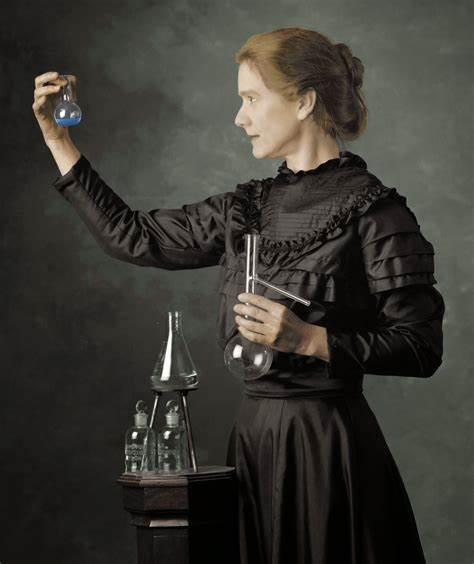
\includegraphics[width=0.38\textwidth]{FQ/Radioatividade/Marie.jpeg}
\caption{Marie Curie}
\end{wrapfigure}

Marie Skłodowska Curie foi uma cientista polonesa com naturalização francesa que conduziu pesquisas pioneiras no ramo da radioatividade. Foi a primeira mulher a ser laureada com um Prémio Nobel e a primeira pessoa e única mulher a ganhar o prêmio duas vezes. Em 1903, Marie dividiu o Nobel de \alert{Física} com o seu marido Pierre Curie e o físico Henri Becquerel. A cientista também foi laureada com o Nobel de \alert{Química} em 1911.

Marie Curie morreu aos 66 anos, em 1934, em um sanatório em Sancellemoz, na França, por conta de uma anemia causada pela exposição a radiação.
\end{frame}





\section{Radiação}
\label{sec:org280c46f}
\begin{frame}[label={sec:org0df0967}]{}
A  radiação  é  a  propagação  de  energia  sob  várias  formas.  Dependendo  da  quantidade de energia, pode ser classificada em não ionizantes e ionizantes

\begin{center}
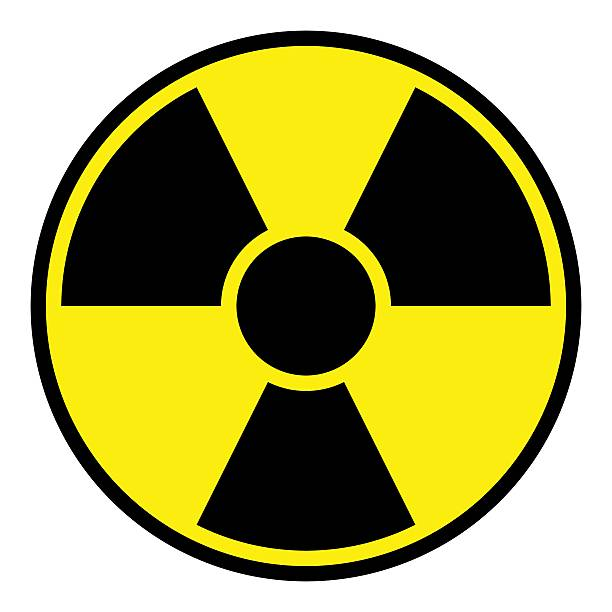
\includegraphics[scale=0.5]{FQ/Radioatividade/RadiacaoSymbol.jpg}
\end{center}
\end{frame}

\begin{frame}[label={sec:org60eb5f6}]{Radiações não ionizantes}
As radiações não ionizantes são caracterizadas por não possuírem energia suficiente para remover elétrons da eletrosfera do átomo, não ocasionando o processo de ionização da matéria. São classificadas de acordo com o compri-mento de onda: ultravioleta, luz visível, infravermelho, micro-ondas e ondas de rádio.  É  importante  ressaltar  que  quanto  menor  o  comprimento  de  onda, maior é a energia da radiação

\begin{figure}[htbp]
\centering
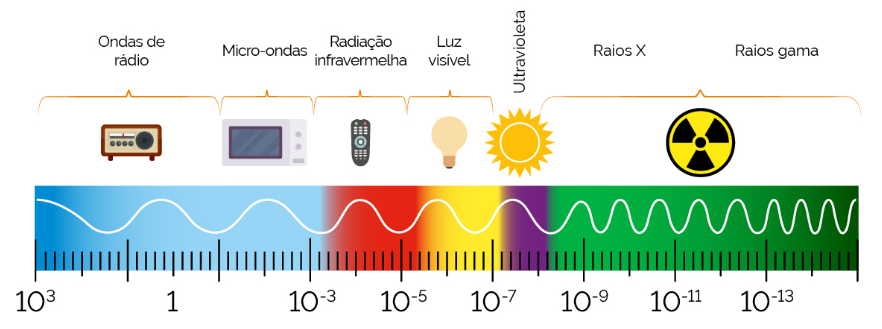
\includegraphics[scale=0.3]{FQ/Radioatividade/espectro.png}
\caption{\label{fig:org1f6003b}Espectro das ondas eletromagnéticas}
\end{figure}
\end{frame}


\begin{frame}[label={sec:org2d3a174}]{Radiações ionizantes}
As radiações ionizantes possuem energia suficiente para provocar a ionização da matéria, ou seja, são capazes de promover a saída de elétrons da eletrosfera dos átomos, podendo causar modificações na estrutura de moléculas e do DNA (Figura ref:ionizado). Estas radiações podem ser corpusculares (partículas alfa e beta) ou ondas eletro-magnéticas (radiação gama).

\begin{figure}[htbp]
\centering
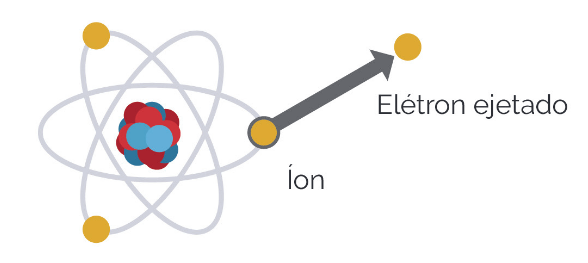
\includegraphics[scale=0.3]{FQ/Radioatividade/ionizado.png}
\caption{\label{fig:orgc8f169a}Processo de ionização.}
\end{figure}
\end{frame}



\begin{frame}[label={sec:org830125a}]{Partículas}
\begin{columns}
\begin{column}{0.45\columnwidth}
\begin{center}


\begin{center}
\begin{tabular}{ll}
\hline
PARTÍCULA & SÍMBOLO\\[0pt]
\hline
PRÓTON & \(\rm _1P^1\)\\[0pt]
NÊUTRON & \(_0n^1\)\\[0pt]
PRÓTIO & \(_1P^1\)\\[0pt]
DEUTÉRIO & \isotope{2,H}\\[0pt]
TRÍTIO & \isotope{3,H}\\[0pt]
PRÓSITON & \(_{+1}^0\upbeta^{+}\)\\[0pt]
\hline
\end{tabular}
\end{center}
\end{center}
\end{column}

\begin{column}{0.45\columnwidth}
\begin{itemize}
\item Emissão de Posítron

\begin{equation*}
 _{+1}^1p \ch{->} _{+1}^{0}\upbeta + _0^{1}n
 \end{equation*}

\item Absorção de um Elétron 

\begin{align*}
  _{+1}^1p \ch{->} _{+1}^{0}\upbeta + _0^{1}n
\end{align*}
\end{itemize}

\begin{center}
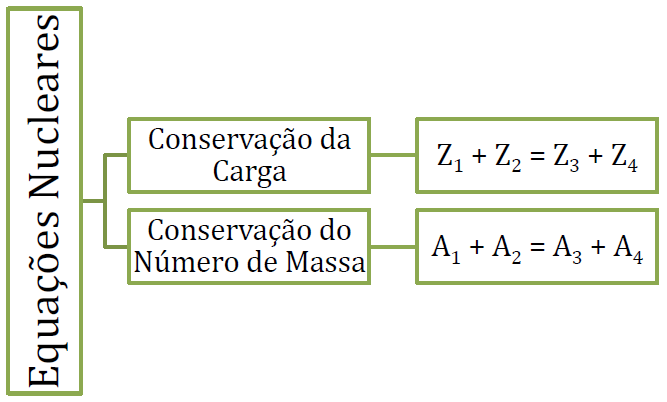
\includegraphics[scale=.2]{FQ/Radioatividade/EqNuclear.png}
\end{center}
\end{column}
\end{columns}
\end{frame}


\begin{frame}[label={sec:orgd2054cb}]{Radiação Alfa (\(\upalpha\))}
\begin{columns}
\begin{column}{0.45\columnwidth}
\begin{tikzpicture}[xscale=0.75,yscale=0.75]
	%axis x
	\definecolor{GreenOlive}{HTML}{006600}	
	\draw [arrows = {-Stealth[length=10pt, inset=5pt]}] (4,0) -- (8,0);
	% axis Y
	\draw [arrows = {-Stealth[length=10pt, inset=5pt]}] (1.0,1) -- (1.0,4);
	%% Text axis x
	\node[draw=none, font=\bfseries] at (8.5,0) {Z};
	%% Text axis Y
	\node[draw=none, font=\bfseries] at (1,4.2) {E};
	%%%%% Linha inferior 
	\draw[line width=1pt] (3,1) --(6,1);
	%% Linha superior 
	\draw [line width=1pt,red] (5,6) --(8,6);
	%\node (a) -- (b);
	\draw[line width=1pt,arrows = {-Stealth[length=10pt, inset=5pt]},GreenOlive] (6.5,6)--(4,1);
	\node(a) at (2.3,1) {\isotope{222,Rn}};
	\node(b) at (8.7,6) {\isotope{226,Ra}};
	\node(c) at (5,4) [font=\bfseries]{$\upalpha$};
\end{tikzpicture}
\end{column}


\begin{column}{0.45\columnwidth}
\begin{itemize}
\item A partícula alfa (\(\alpha\)) é composta por dois prótons e dois nêutrons (núcleo de hélio), é emitida com alta energia e possui baixo poder de penetração e alto poder ionizante.
\item São emissões típicas de átomos com alto peso atômico.
\item Esse tipo de radiação tem grande importância na medicina para o tratamento de doenças, como o câncer.
\item Exemplos de radionuclídeos emissores de alfa: rádio-223 (\(^{223}\)Ra), urânio-238 (\(^{238}\)U), plutônio-239 (\(^{239}\)Pu).
\end{itemize}
\end{column}
\end{columns}
\end{frame}


\begin{frame}[label={sec:org3233021}]{Beta (\(\upbeta^-\))}
\begin{columns}
\begin{column}{0.45\columnwidth}
\begin{tikzpicture}[xscale=.75,yscale=.75]
	%axis x
	\definecolor{GreenOlive}{HTML}{006600}	
	\draw [arrows = {-Stealth[length=10pt, inset=5pt]}] (4,0) -- (8,0);
	% axis Y
	\draw [arrows = {-Stealth[length=10pt, inset=5pt]}] (2,1) -- (2,4);
	%% Text axis x
	\node[draw=none, font=\bfseries] at (8.5,0) {Z};
	%% Text axis Y
	\node[draw=none, font=\bfseries] at (2,4.2) {E};
	%%%%% Linha inferior 
	\draw[line width=1pt] (5,1) --(8,1);
	%% Linha superior 
	\draw [line width=1pt,red] (3,6) --(6,6);
	%\node (a) -- (b);
	\draw[line width=1pt,arrows = {-Stealth[length=10pt, inset=5pt]},GreenOlive] (4.5,6)--(6.5,1);
	\node(a) at (8.5,1) {\isotope{14,N}};
	\node(b) at (6.5,6) {\isotope{14,C}};
	\node(c) at (5,4) [font=\bfseries]{$\upbeta^-$};
\end{tikzpicture}
\end{column}

\begin{column}{0.45\columnwidth}
\small

\begin{itemize}
\item A radiação beta é subdividida em dois tipos, beta menos (\(\upbeta ^-\)) e pósitron (\(\upbeta ^+\)). As emissões do tipo \(\upbeta ^-\)- possuem a mesma característica dos elétrons atômicos, com a diferença que sua origem se dá no núcleo que possui um número excessivo de nêutrons sendo, portanto, instável.
\item Neste decaimento o nêutron se “transforma” em um elétron (ejetado) e um próton (este permanece no núcleo). Assim como a  radiação  alfa,  elementos  emissores  de  beta  menos  (\(\upbeta ^-\))  podem  ser  usados  no  tratamento de doenças. Exemplos: lutécio-177 ( \ch{^{177}Lu}),  ítrio-90 (\ch{^{90}Y}).
\end{itemize}
\end{column}
\end{columns}
\end{frame}

\begin{frame}[label={sec:orge739c11}]{Pósitron (\(\upbeta^+\))}
\begin{columns}
\begin{column}{0.45\columnwidth}

\begin{tikzpicture}[xscale=.75,yscale=.75]
	%axis x
\definecolor{GreenOlive}{HTML}{006600}	
\draw [arrows = {-Stealth[length=10pt, inset=5pt]}] (4,0) -- (8,0);
% axis Y
\draw [arrows = {-Stealth[length=10pt, inset=5pt]}] (2,1) -- (2,4);
%% Text axis x
\node[draw=none, font=\bfseries] at (8.5,0) {Z};
%% Text axis Y
\node[draw=none, font=\bfseries] at (2,4.2) {E};
%%%%% Linha inferior 
\draw[line width=1pt] (3,1) --(6,1);
%% Linha superior 
\draw [line width=1pt,red] (5,6) --(8,6);
%\node (a) -- (b);
\draw[line width=1pt,arrows = {-Stealth[length=10pt, inset=5pt]},GreenOlive] (6.5,6)--(4,1);
\node(a) at (2.5,1) {\isotope{N}};
\node(b) at (8.5,6) {\isotope{14,O}};
\node(c) at (5,4) [font=\bfseries]{$\upbeta^+$};
\end{tikzpicture}
\end{column}


\begin{column}{0.45\columnwidth}
\small\{
\begin{itemize}
\item Outro tipo de emissão beta é o pósitron (\(\upbeta ^+\)), que consiste na transformação de  um  próton  em  nêutron  e  pósitron  (antielétron),  uma  vez  que  o  núcleo  se  encontra  instável  devido  ao  número  elevado  de  prótons.
\item Após  sua  emissão  do  núcleo, os pósitrons são quase que instantaneamente aniquilados dando origem a dois fótons com mesma energia (511 keV) e direções opostas. Esse tipo de radiação é utilizado na medicina diagnóstica. Exemplo de radionuclídeos emissores de pósitrons: gálio-68  (\ch{^{68}Ga}), flúor-18 (\ch{^{18}F}).
\end{itemize}
\}
\end{column}
\end{columns}
\end{frame}

\begin{frame}[label={sec:orgb6f9eb5}]{Radiação Gama}
\small\{
   A radiação \alert{gama} (\(\gamma\)) é conceituada como ondas eletromagnéticas emitidas do núcleo de um átomo. Apresenta energia superiores e alto poder de penetração, enquanto que os raios X são menos energéticos. Exemplo de radionuclídeos emissores de radiação gama:  \ch{^{99m}Tc}, cobalto-60 (\ch{^{60}Co}).
\}



\begin{columns}
\begin{column}{0.45\columnwidth}
\begin{tikzpicture}[xscale=.75,yscale=.75]
	%\begin{tikzpicture}
	%axis x
	\definecolor{GreenOlive}{HTML}{006600}	
	\definecolor{Purple}{HTML}{800080}
	\definecolor{VioletRed}{HTML}{c71585}
	%%%%% Linha inferior 
	\draw[line width=1.5pt,Purple] (5,1) --(8,1);
	\draw[line width=1.5pt,blue] (5,0) --(8,0);
	%% Linha superior 
	\draw [line width=1.5pt,red] (3,6) --(6,6);
	%\node (a) -- (b);
	\draw[line width=1pt,arrows = {-Stealth[length=10pt, inset=5pt]},GreenOlive] (4.5,6)--(6.5,1);
	\node(a) at (8.8,1) {\isotope{18,Ar}$^*$};
	\node(a2) at (8.8,0) {\isotope{18,Ar}};
	\node(b) at (6.8,6) {\isotope{38,Cl}};
	\node(c) at (6.1,4) [font=\bfseries]{$\upbeta^-$};
	\draw [->,decorate,decoration={snake,amplitude=.4mm,segment length=2mm,post length=2mm},VioletRed] (7,1) --(7,0);
	\node(d) at (7.4,0.5) [font=\bfseries]{$\upgamma$};
\end{tikzpicture}
\end{column}


\begin{column}{0.45\columnwidth}

\begin{reaction*}
	\isotope{Ra} -> \isotope{Rn} + $\upalpha$
\end{reaction*}


\begin{tikzpicture}[xscale=0.75,yscale=0.75]
	%axis x
	\definecolor{GreenOlive}{HTML}{006600}
	\definecolor{Purple}{HTML}{800080}
	\definecolor{VioletRed}{HTML}{c71585}
%	\draw [arrows = {-Stealth[length=10pt, inset=5pt]}] (4,0) -- (8,0);
	% axis Y
%	\draw [arrows = {-Stealth[length=10pt, inset=5pt]}] (1.0,1) -- (1.0,4);
	%% Text axis x
%	\node[draw=none, font=\bfseries] at (8.5,0) {Z};
	%% Text axis Y
%	\node[draw=none, font=\bfseries] at (1,4.2) {E};
	%%%%% Linha inferior 
	\draw[line width=1.5pt,Purple] (2,1) --(6,1);
	\draw[line width=1.5pt,blue] (2,0) --(6,0);
	%% Linha superior 
	\draw [line width=1.5pt,red] (5,6) --(9,6);
	%\node (a) -- (b);
	\draw[line width=1pt,arrows = {-Stealth[length=10pt, inset=5pt]},GreenOlive] (7,6)--(4,1);
	\draw[line width=1pt,arrows = {-Stealth[length=10pt, inset=5pt]},GreenOlive] (8.5,6)--(6.,0);
	\node(a) at (1.,1) {\isotope{222,Rn}$^*$};
	\node(a) at (1,0) {\isotope{222,Rn}};
	\node(b) at (9.7,6) {\isotope{226,Ra}};
	\node(c) at (5,4) [font=\bfseries]{$\upalpha$};
	\node(c1) at (8,3.5) [font=\bfseries]{$\upalpha$};
	\draw [->,decorate,decoration={snake,amplitude=.4mm,segment length=2mm,post length=2mm},VioletRed] (4,1) --(4,0);
	\node(d) at (4.4,0.5) [font=\bfseries]{$\upgamma$};
\end{tikzpicture}
\end{column}
\end{columns}
\end{frame}




\begin{frame}[label={sec:org8dd48a8}]{Poder de penetração da radiação}
Com isso, os radionuclídeos emissores de alfa e beta podem ser utilizados na terapia de doenças e os emissores de gama, no diagnóstico.
\vspace{0.0cm}
\begin{figure}[H]
\centering
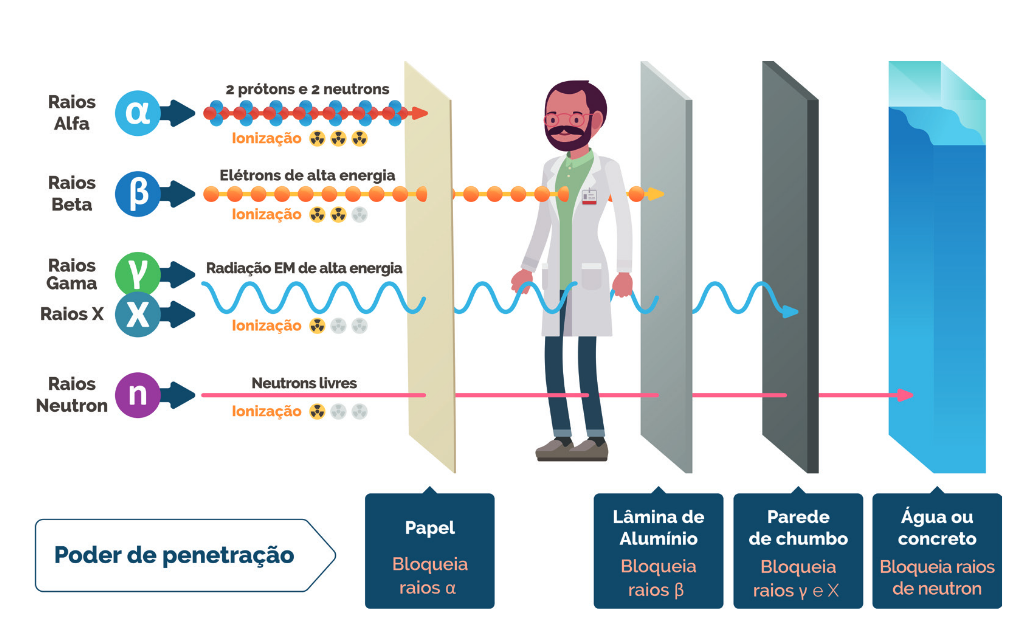
\includegraphics[scale=0.28]{FQ/Radioatividade/poder.png}
\caption{\label{fig:orgdb66ddd}Poder de penetração das radiações.}
\end{figure}
\end{frame}



\section{Radionuclídeos}
\label{sec:org2bdef84}

\begin{frame}[label={sec:org2825bb8}]{Radionuclídeos}
Os radionuclídeos podem ser encontrados na natureza, como o  \ch{^238{U}} e o \ch{^{233}Ra}, ou podem ser produzidos artificialmente, de forma direta, em reatores nucleares e cíclotrons, ou de forma indireta, por geradores. O radionuclídeo é um átomo considerado instável em função de seu núcleo possuir energia “em excesso”.

\begin{figure}[H]
\centering
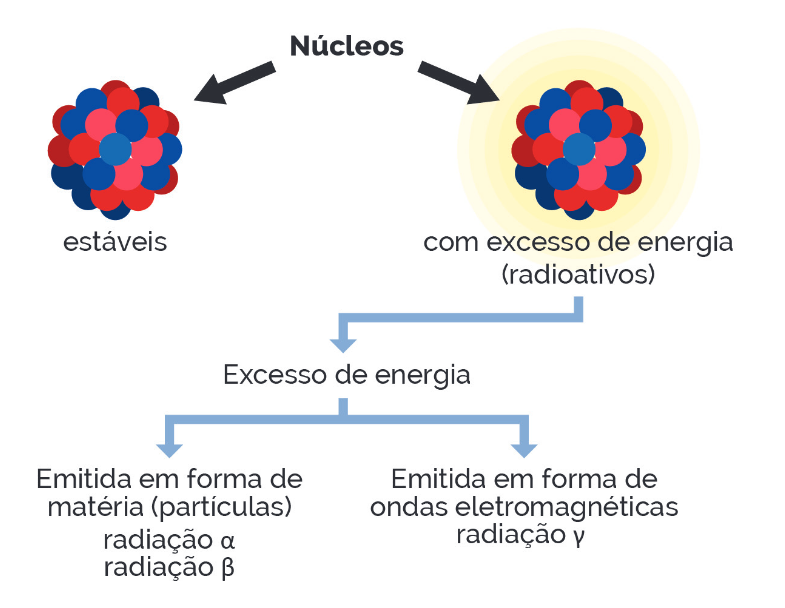
\includegraphics[scale=0.24]{FQ/Radioatividade/nucleo.png}
\caption{\label{fig:org04c6a03}Processo de desintegração do radionuclídeo.}
\end{figure}
\end{frame}


\section{Meia-vida}
\label{sec:org2583f5b}

\begin{frame}[label={sec:orgb153a58}]{Meia-vida física}
Meia-vida física (\(t_{\frac{1}{2}}\)) corresponde ao tempo necessário para a atividade inicial de um elemento radioativo ser reduzida à metade por meio de seu decaimento e consequente emissão de radiação. A meia-vida de um radionuclídeo pode variar de poucos segundos a vários anos.



\begin{columns}
\begin{column}{0.45\columnwidth}
\begin{equation}
%t_{\frac{1}{2}}= \frac{0,693}{k}
m=\frac{m_0}{2^x}
\end{equation}

\begin{equation}
t=x\cdot P
\end{equation}

\begin{description}
\item[{\(m\)}] massa final
\item[{\(m_o\)}] massa inicial
\item[{\(x\)}] número de períodos de meia-vida (x)
\item[{\(P\)}] período da meia-vida
\item[{\(t\)}] tempo de desintegração
\end{description}
\end{column}



\begin{column}{0.45\columnwidth}
\begin{figure}[H]
\centering
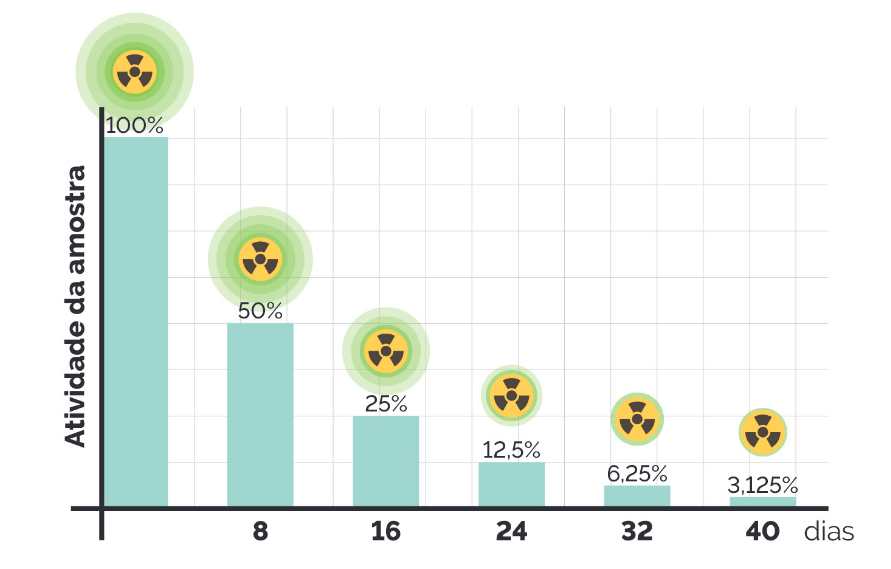
\includegraphics[scale=0.21]{FQ/Radioatividade/meia-vida.png}
\caption{\label{fig:orgf422151}Decaimento do  \isotope{131,I}  pela sua meia-vida física de 8 dias.}
\end{figure}
\end{column}
\end{columns}
\end{frame}

\begin{frame}[label={sec:orgbf1d788}]{Meia-vida biológica e efetiva}
A meia-vida biológica representa o tempo necessário para que o organismo excrete 50\% do fármaco. Quando se trata de radiofármacos, é necessário levar em conta também a meia-vida efetiva, que é a soma da meia-vida física e a meia-vida biológica.

A atividade de uma amostra é definida pelo número de desintegrações por segundo do núcleo instável de um radionuclídeo. Dessa forma, é possível mensurar a radioatividade de uma amostra. 
\end{frame}

\begin{frame}[label={sec:orgbc8d485}]{}
\vspace{-1cm}

\begin{question}
\small\{
Um radioisótopo utilizado no tratamento radioterápico apresenta uma meia-vida (período de semidesintegração) de 5 horas. Se um técnico utilizar uma massa de 50 g no tratamento de um paciente, após quantas horas a massa seria reduzida para 6,25 g?

a) 5 horas.  \quad b) 25 horas. \quad c) 15 horas. \quad d) 30 horas. \quad e) 10 horas.

\}
\begin{myrule}{Solução}
\begin{minipage}{0.5\textwidth}


\alert{1º Passo:} Calcular o número de meias-vidas que foram necessárias para a redução de 50 g para 6,25 g por meio da fórmula a seguir.

\begin{align*}
m=\frac{m_0}{2^x} \\
6,25 = \frac{50}{2^x}\\
2^x= \frac{50}{6,25}\\
2^x=8 \\
2^x = 2^3 \\
x= 3
\end{align*}
3 meias-vidas
\end{minipage}
\hspace{0.05\textwidth}
\begin{minipage}{0.4\textwidth}
\alert{2º Passo:} Em seguida, para calcular o tempo, basta utilizar a seguinte expressão:
\begin{align*}
t = x \cdot P \\
t = 5 \cdot 3 \\
t = 15 ~ \text{h}
\end{align*}
\end{minipage}
\end{myrule}
\end{question}
\end{frame}


\section{Reação Nuclear}
\label{sec:org0b6f2bc}

\begin{frame}[label={sec:orgbd2d1e4}]{Reação Nuclear}
É a propriedade que os núcleos instáveis possuem de emitir partículas e radiações eletromagnéticas, para se tornarem estáveis


A radioatividade natural ocorre, geralmente, com os átomos de números atômicos maiores que 82


A reação que ocorre nestas condições, isto é, alterando o núcleo do átomo chama-se \alert{REAÇÃO NUCLEAR}
\end{frame}


\section{Decaimento Radioativo}
\label{sec:org635dc3b}


\begin{frame}[label={sec:org41a43de}]{Lei de Soddy}
\alert{Decaimento alfa:} nela, o núcleo instável emite uma partícula alfa, que é um núcleo de Hélio. Como sabemos da tabela periódica, o Hélio tem dois prótons e dois nêutrons. Assim, o elemento perde 4 de massa, tendo seu número atômico diminuído em 2.

\begin{center}
  \ch{^A_Z X -> ^4_2\(\alpha\) + ^{A-4}_{Z-2}Y} 
\end{center}

\begin{center}
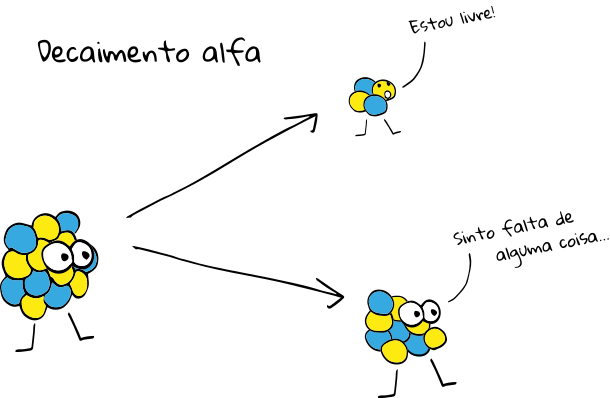
\includegraphics[scale=0.2]{FQ/Radioatividade/alfa.png}
\end{center}
\end{frame}

\begin{frame}[allowframebreaks,label=]{Lei de Soddy, Fajans e Russel}
\alert{Decaimento beta:} a partícula beta é um elétron ejetado de um nêutron. Como elétrons não têm massa, ela também não tem. O elemento radioativo tem um nêutron transformado em próton, então aumenta seu número atômico em 1.

\begin{center}
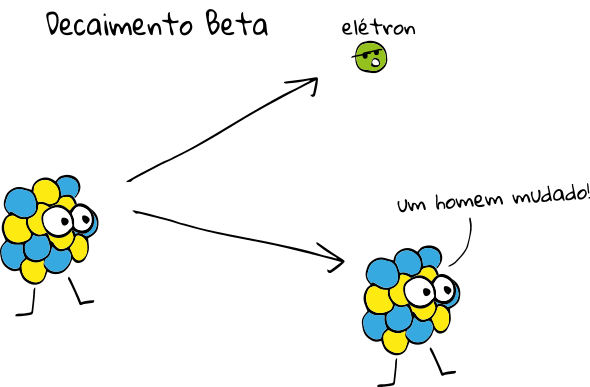
\includegraphics[scale=0.2]{FQ/Radioatividade/beta.png}
\end{center}

\begin{bclogo}[logo=\bcinfo]{Decaimento Beta}
\ch{^A_Z Q -> ^0_{-1} \(\beta\) + ^{A-0}_{Z+1}R}
\begin{tikzpicture}[xscale=.6]
 \shade[ball color=blue] (0,0) circle (6ex);
 \node[draw=none,align=left,font=\bfseries] at (0,1.3) {Nêutron};
 \node[draw=none,align=left,font=\bfseries] at (3,0) {\ch{->[Decaimento ~ $\upbeta^-$]}};
\shade[ball color=red] (6,0) circle (6ex);
 \node[draw=none,align=left,font=\bfseries] at (6,1.3) {Próton};
 \shade[ball color=yellow] (10,0) circle (6ex);
\node[draw=none,align=left,font=\bfseries] at (10,1.3) {elétron};
\node[draw=none,align=left,font=\bfseries] at (8.,0) {+};
 \shade[ball color=teal] (14,0) circle (6ex);
 \node[draw=none,align=left,font=\bfseries] at (12.,0) {+};
 \node[draw=none,align=left,font=\bfseries] at (14.,1.3) {antineutrino};
\end{tikzpicture}
\end{bclogo}

\alert{Decaimento Pósitron}: No decaimento de pósitrons , perdemos uma carga positiva do núcleo. Isso significa que o número atômico diminuirá em uma unidade.

\begin{bclogo}[logo=\bcinfo]{Decaimento Positron}
\begin{tikzpicture}[xscale=0.6]
	\shade[ball color=red] (0,0) circle (6ex);
	\node[draw=none,align=left,font=\bfseries] at (0,1.3) {Próton};
	\node[draw=none,align=left,font=\bfseries] at (3,0) {\ch{->[Decaimento ~ $\upbeta^+$]}};
	\shade[ball color=blue] (6,0) circle (6ex);
	\node[draw=none,align=left,font=\bfseries] at (6,1.3) {Nêutron};
	\shade[ball color=gray] (10,0) circle (6ex);
	\node[draw=none,align=left,font=\bfseries] at (10,1.3) {pósitron};
	\node[draw=none,align=left,font=\bfseries] at (8.,0) {+};
	\shade[ball color=green] (14,0) circle (6ex);
	\node[draw=none,align=left,font=\bfseries] at (12.,0) {+};
	\node[draw=none,align=left,font=\bfseries] at (14.,1.3) {neutrino};
\end{tikzpicture}
\end{bclogo}
\end{frame}

\begin{frame}[label={sec:orgb1c7711}]{Radiação Gamma}
\begin{center}
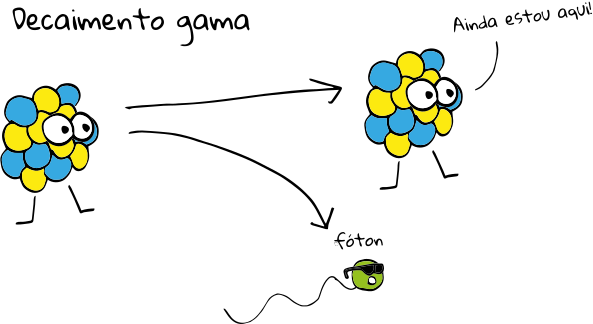
\includegraphics[scale=.3]{FQ/Radioatividade/gama.png}
\end{center}
\end{frame}



\begin{frame}[label={sec:org8451eb1}]{}
\vspace{-1cm}
\begin{question}{Exemplo}
\small
Ao se desintegrar, o átomo \isotope{222,Rn} emite 3 partículas alfa e 4 partículas beta. O nº atômico e o nº de massa do átomo final são, respectivamente:

a) 84 e 210. \qquad     b) 210 e 84.  \qquad    c) 82 e 210. \qquad    d) 210 e 82. \qquad    e) 86 e 208.

\begin{myrule}{Solução}


\begin{align*}
\isotope{222,Rn} \ch{->} 3 \cdot  \upalpha_2^4 \quad  +  \quad 4 \cdot_{-1}\upbeta^0 \quad + \quad  \rm{}_Z^AX
\end{align*}

\begin{columns}[T] % align columns
\begin{column}{.48\textwidth}
\color{red}\rule{\linewidth}{4pt}

\begin{align*}
	86 = & 3 \cdot 2 + 4 \cdot (– 1) + Z \\
	86 = & 6 – 4 + Z \\
	Z = & 86 – 2 \\
	Z = & 84
\end{align*}

\end{column}%
\hfill%
\begin{column}{.48\textwidth}
\color{blue}\rule{\linewidth}{4pt}

\begin{align*}
222 = 3 \cdot 4 + 4\cdot 0 + A \\
222 = 12 + A \\
A = 222 – 12 \\ 
A = 210 \\ 
\end{align*}
\end{column}%
\end{columns}
\end{myrule}
\end{question}
\end{frame}





\section{Séries Radioativas}
\label{sec:org2452dae}

\begin{frame}[label={sec:orged4658a}]{Séries Radioativas}
\begin{itemize}
\item É o conjunto de elementos que têm origem na missão de partículas alfa e beta, resultando, como elemento final, um isótopo estável do chumbo.
\end{itemize}
\begin{center}
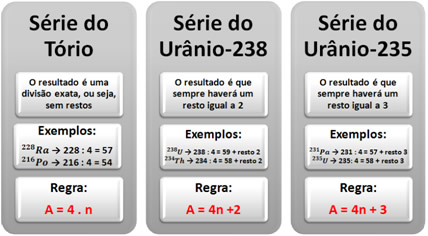
\includegraphics[width=.9\linewidth]{FQ/Radioatividade/serieradioativas.jpg}
\end{center}
\end{frame}

\section{Fissão Nuclear}
\label{sec:org4fcdc1f}
\begin{frame}[label={sec:org516efbf}]{Fissão Nuclear}
A \alert{fissão nuclear} é caracterizada pelo processo de quebra de núcleos grandes em núcleos menores, provocando a liberação de uma grande quantidade de energia.


\begin{tikzpicture}[xscale=0.7,yscale=0.7]
\begin{scope}
		\shade[ball color=white] (-5,0) circle (2ex);
		\node[draw=none,align=left,font=\bfseries] at (-5,0.75) {nêutron};
		\draw[line width=1pt,arrows = {-Stealth[length=10pt, inset=5pt]}] (-4,0)--(-1.5,0);
		\node[starburst, fill=yellow, draw=red, line width=2pt,font=\bfseries] at (4,0){ Energia};
		\draw[line width=1pt,arrows = {-Stealth[length=10pt, inset=5pt]}] (1.5,0)--(4,2);
		\draw[line width=1pt,arrows = {-Stealth[length=10pt, inset=5pt]}] (1.5,0)--(3.5,-2.5);
		\shade[ball color=white] (7,1.5) circle (2ex);
		\shade[ball color=white] (7,0) circle (2ex);
		\shade[ball color=white] (7,-1.5) circle (2ex);
\end{scope}
%%%%% Uranio
\begin{scope}[local bounding box=scope1]
		\path (-2,-2) rectangle (2,2);
	\pgfmathdeclarerandomlist{color}{{red}{white}}
	\pgfmathsetseed{1}
	\foreach \A/\R in {25/1,12/0.9,15/0.8,20/0.7,12/0.5,7/0.3,1/0}{
		\pgfmathsetmacro{\S}{360/\A}
		\foreach \B in {0,\S,...,360}{
			\pgfmathrandomitem{\C}{color}
			\shade[ball color=\C] (\B+\A:\R) circle (7pt);
		}
	}
	\node[draw=none,align=left,font=\bfseries] at (-1,1.3) {\isotope{235,U}};
\end{scope}
\begin{scope}[shift={($(scope1.east)+(3cm,3)$)}]
		\path (-2,-2) rectangle (2,2);
	\pgfmathdeclarerandomlist{color}{{red}{white}}
	\pgfmathsetseed{1}
	\foreach \A/\R in {25/1,12/0.9,15/0.8,20/0.7,12/0.5,7/0.3,1/0}{
		\pgfmathsetmacro{\S}{360/\A}
		\foreach \B in {0,\S,...,360}{
			\pgfmathrandomitem{\C}{color}
			\shade[ball color=\C] (\B+\A:\R) circle (3.5pt);
		}
	}
	\node[draw=none,align=left,font=\bfseries] at (-1,1.3) {\isotope{139,Ba}};
\end{scope}
\begin{scope}[shift={($(scope1.east)+(3cm,-3)$)}]
	\path (-2,-2) rectangle (2,2);
	\pgfmathdeclarerandomlist{color}{{red}{white}}
	\pgfmathsetseed{1}
	\foreach \A/\R in {25/1,12/0.9,15/0.8,20/0.7,12/0.5,7/0.3,1/0}{
		\pgfmathsetmacro{\S}{360/\A}
		\foreach \B in {0,\S,...,360}{
			\pgfmathrandomitem{\C}{color}
			\shade[ball color=\C] (\B+\A:\R) circle (3.pt);
		}
	}
	\node[draw=none,align=left,font=\bfseries] at (-1,1.3) {\isotope{95,Kr}};
\end{scope}
\end{tikzpicture}
\end{frame}

\section{Fusão Nuclear}
\label{sec:org1eeef8d}
\begin{frame}[label={sec:org688f340}]{Fusão Nuclear}
A \alert{fusão nuclear} é uma reação nuclear na qual dois núcleos de átomos leves se unem para formar outro núcleo mais pesado. 

\begin{tikzpicture}[xscale=.75,yscale=.75]
	
	\node[align=center,font=\bfseries] at (-5,1) {Deutério};
	\node[align=center,font=\bfseries] at (-5,-4) {Trítio};
	%%%% Line Deuterio
	 \draw[line width=1pt,arrows = {-Stealth[length=10pt, inset=5pt]}] (-4.5,0)--(-1,-1);
	 %%% Line Tritio
	 \draw[line width=1pt,arrows = {-Stealth[length=10pt, inset=5pt]}] (-4.5,-3)--(-1,-2);
	 %%%% Line Helio
	 \draw[line width=1pt,arrows = {-Stealth[length=10pt, inset=5pt]}] (3,-2)--(5.5,-3);
	 \node[draw=none,align=left,font=\bfseries] at (6.3,-4.3) {\isotope{He}};
	 % Line Neutron 
	 \draw[line width=1pt,arrows = {-Stealth[length=10pt, inset=5pt]}] (3,-1)--(5.6, 0.4);
	 \node[draw=none,align=left,font=\bfseries] at (5.5,1.3) {nêutron};
	 %%% Line Energia
	 \draw[line width=1pt,arrows = {-Stealth[length=10pt, inset=5pt]}] (2.5, -1.5)--(7, -1.5);
	 \node[starburst, fill=yellow, draw=red, line width=2pt,font=\bfseries] at (9.3,-1.5){Energia};
\begin{scope}[local bounding box=scope1]
	\shade[ball color=white] (-5,0) circle (2ex);
	\shade[ball color=red] (-5,0.5) circle (2ex);
\end{scope}
\begin{scope}[local bounding box=scope2,shift={($(scope1.south)+(5cm,-3)$)},anchor=below]
	\shade[ball color=white] (-5,0) circle (2ex);
	\shade[ball color=red] (-5,0.5) circle (2ex);
	\shade[ball color=white] (-5,1) circle (2ex);
\end{scope}
\begin{scope}[local bounding box=scope3,shift={($(scope2.west)+(8cm,1.5)$)}]
	\node[starburst, fill=yellow, draw=red, line width=2pt,font=\bfseries] at (-2,0){
\begin{tikzpicture}
	\shade[ball color=white] (-4.9,1.0) circle (2ex);
	\shade[ball color=white] (-4.4,0.7) circle (2ex);
	\shade[ball color=white] (-5,0) circle (2ex);
	\shade[ball color=red] (-5,0.5) circle (2ex);
	\shade[ball color=red] (-4.5,0.3) circle (2ex);
\end{tikzpicture}
};
\end{scope}
\begin{scope}[local bounding box=scope4,shift={($(scope3.west)+(12cm,-2)$)}]
%\shade[ball color=white] (-4.9,1.0) circle (2ex);
\shade[ball color=white] (-4.4,0.7) circle (2ex);
\shade[ball color=white] (-5,0) circle (2ex);
\shade[ball color=red] (-5,0.5) circle (2ex);
\shade[ball color=red] (-4.5,0.3) circle (2ex);
\end{scope}
\begin{scope}[local bounding box=scope4,shift={($(scope3.west)+(12cm,2)$)}]
	\shade[ball color=white] (-5,0) circle (2ex);
\end{scope}
\end{tikzpicture}
\end{frame}

\section{Aplicação}
\label{sec:org57494ea}
\begin{frame}[label={sec:org94a2b83}]{Radioterapia}
A \alert{radioterapia} é um tratamento no qual se utilizam radiações ionizantes (raio-X, por exemplo), um tipo de energia direcionada, para destruir ou impedir que as células do tumor aumentem.

\begin{center}
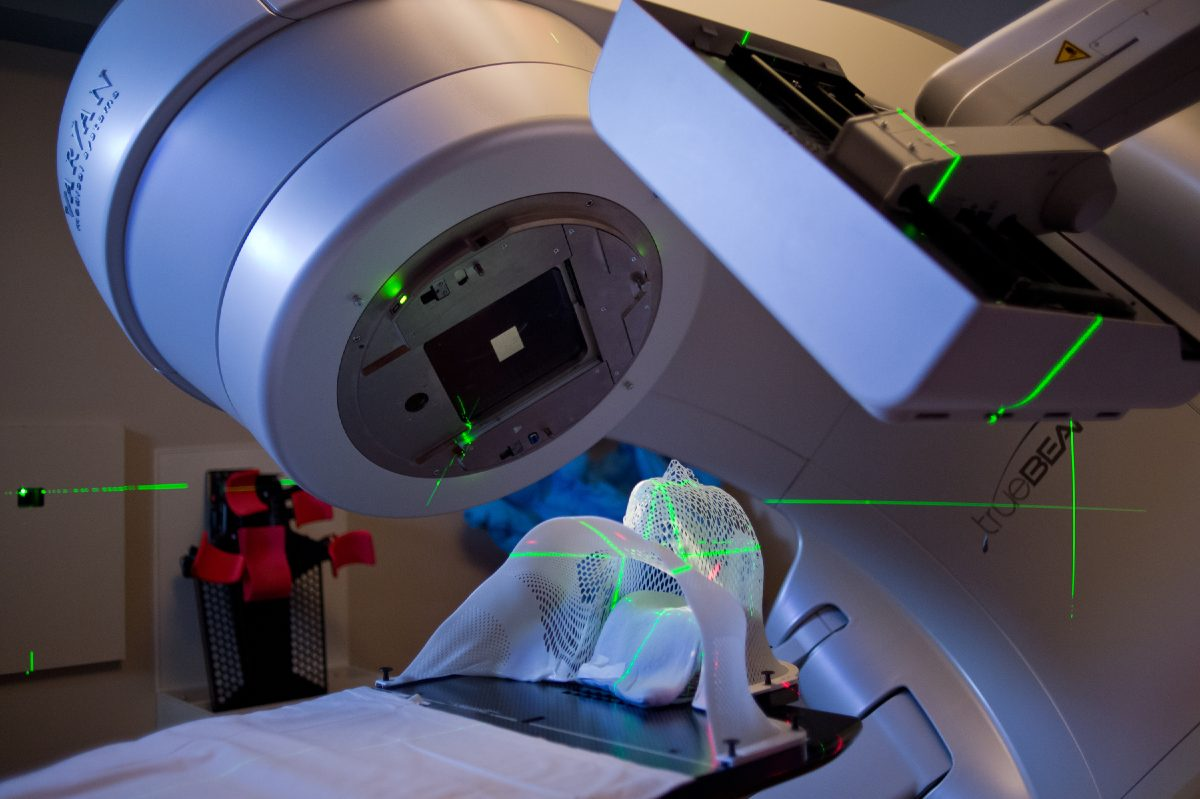
\includegraphics[scale=.8]{FQ/Radioatividade/radioterapia.jpg}
\end{center}
\end{frame}

\begin{frame}[label={sec:orgef46751}]{Radiofármacos}
O Tabela mostra os radiofármacos mais utilizados para tratamentos específicos. Para cada caso há um tempo de exposição e uma dose que varia de fração de segundos a horas.



\begin{table}[htbp]
\caption{\label{tab:orgd6d9b09}Radiofármacos específicos  para tratamento}
\centering
\begin{tabular}{|c|c|}
\hline
\alert{Radiofármaco} & \alert{Tratamento}\\[0pt]
\hline
IODO ( \isotope{131,I}) & Tumores de tiroíde, fígado e rins\\[0pt]
\hline
CROMO ( \isotope{51,Cr}) & Trato de patologias intestinais\\[0pt]
\hline
GÁLIO ( \isotope{67,Ga}) & Tumores em tecidos moles.\\[0pt]
\hline
TECNÉSIO ( \isotope{99,Tc}) & Tumores de cérebro, glândulas salivares, coração\\[0pt]
\hline
GADOLÍNIO ( \isotope{159,Gd}) & estomâgo, sistema ósseo, fígado, rins, pulmão\\[0pt]
\hline
\end{tabular}
\end{table}
\end{frame}

\begin{frame}[label={sec:orgcbe9fdd}]{Fim da Aula}
\begin{tikzpicture}
\node[graduate,sword, devil, minimum size=1cm]{ \bfseries Bons Estudos !!!!};
\end{tikzpicture}
\begin{center}
\begin{tabular}{ccc}
Download Aula & & Lista de Exercícios \\
 \qrcode[height=2in]{https://github.com/fabinholima/AulaQuimicaPDF/blob/main/FQ/Radioatividade/Radioatividade.pdf} & & \qrcode[height=2in]{https://github.com/fabinholima/AulaQuimicaPDF/blob/main/FQ/Radioatividade/Lista_Radioatividade.pdf}\\
 \end{tabular}
 \end{center}
\end{frame}

\begin{frame}[label={sec:org68cf174}]{Recomendações}
\begin{block}{Filme}
Radioatividade 
\url{https://www.netflix.com/br/title/81168940}
\end{block}

\begin{block}{Documentário}
O brilho da morte 
\url{https://youtu.be/gCcTxnvZb-k?si=ITvRVFqsry2oGc1A}
\end{block}
\end{frame}
\end{document}
